\section{Assignment 7}
\subsection{Feature selection}

Before starting to solve the clusterization problem we decided to do empirical feature selection to get more inpretable and more clear-cut data structure. 
After some attempts we have choosen:
\begin{itemize}
\item
Channel-type nominal features

\begin{itemize}
\item
\texttt{data\_channel\_is\_lifestyle}, \\
\texttt{data\_channel\_is\_entertainment}, \\ 
\texttt{data\_channel\_is\_bus}, \\ 
\texttt{data\_channel\_is\_socmed}, \\
\texttt{data\_channel\_is\_tech}, \\
\texttt{data\_channel\_is\_world} (all are logical).

\item
\texttt{channel} (numeric from 0 to 6)
\end{itemize}
\item
Some words characteristics

\begin{itemize}
\item
\texttt{n\_tokens\_title}, \\
\texttt{n\_tokens\_content}, \\
\texttt{n\_unique\_tokens}, \\
\texttt{average\_token\_length}, \\
\texttt{num\_keywords} (numeric).
\end{itemize}
\end{itemize}

We have also logarithmed all log-normal features.
Unlike previous assignments we haven't deleted zero-length articles to classify them as individual cluster.

\subsection{K-Means Clustering}

First of all we have plotted PCA-plot of our data, you can see the results at Figure \ref{fig:k-means}. One can find 2,7 or some other number of clusters. 

Then we applied built-in function \texttt{kmeans} with parameters $k=3,4,7$ and multi-start with $\texttt{nstart = 100}$, the results of this clusterization are presented at Figure \ref{fig:k-means}.
We should notice that left-bottom cluster in all plots is rather far from the other clusters. During the data analysis we have found out that these points match zero-length articles.  

\begin{figure}[h]
	\centering
	\begin{minipage}[h]{0.49\linewidth}
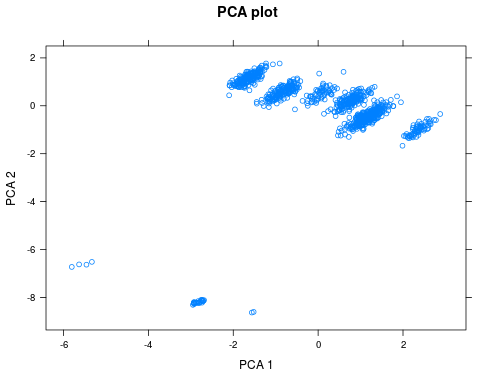
\includegraphics[width=\linewidth]{images/pcaplot_km}
	\end{minipage}
	\hfill
	\begin{minipage}[h]{0.49\linewidth}
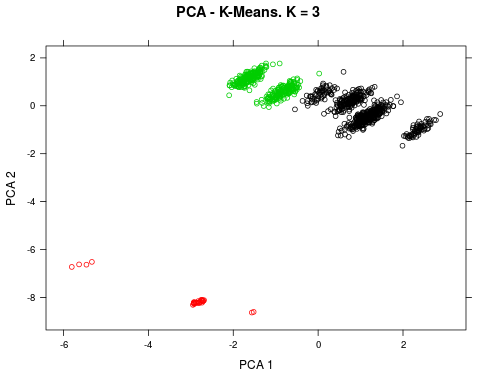
\includegraphics[width=\linewidth]{images/kmean3}
	\end{minipage}
	\begin{minipage}[h]{0.49\linewidth}
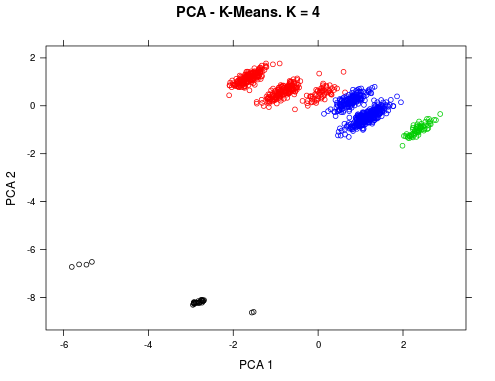
\includegraphics[width=\linewidth]{images/kmean4}
	\end{minipage}
	\hfill
	\begin{minipage}[h]{0.49\linewidth}
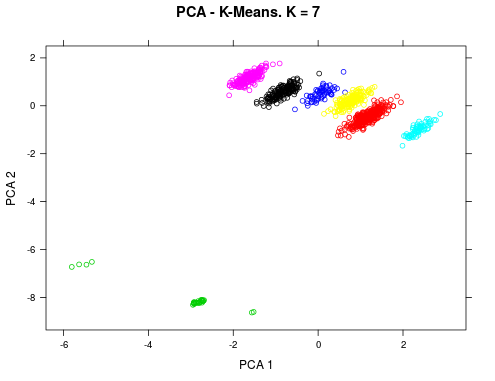
\includegraphics[width=\linewidth]{images/kmean7}
	\end{minipage}
	\caption{PCA plot without clusterization (a), with k-means clusterization with $k=3,4,7$}
	\label{fig:k-means}
\end{figure} 

As we know, k-means method is minimizing the value of total within-cluster sum of squares distance to cluster mean. 
In order to find the optimum number of clusters, we have built plot 
`total within-cluster sum of squares' to `number of clusters' (see Figure {\ref{fig:totalwithin-to-k}).

\begin{figure}[h]
	\centering
	\begin{minipage}[h]{0.49\linewidth}
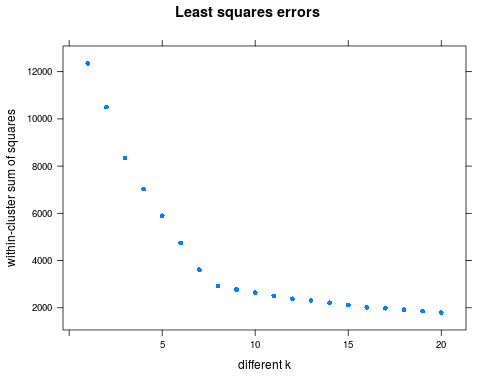
\includegraphics[width=\linewidth]{images/totalwithin}
	\end{minipage}
	\caption{Dependence between `total within-cluster sum of squares' and `number of clusters'}
	\label{fig:totalwithin-to-k}	
\end{figure}

As we can see from the plot, the optimal number of clusters is about 7 (or 8, if we want to divide left-bottom cluster into two parts).

\subsection{Nearest Neighbor clustering with MST}



